\section{Use Case}\label{sec:UseCase}
The proposed techinque, \tech is tested in the simulator SUMO on a part of Hobrovej, which is a frequently used road in Aalborg, Denmark.

\begin{figure}[htb]
\centering
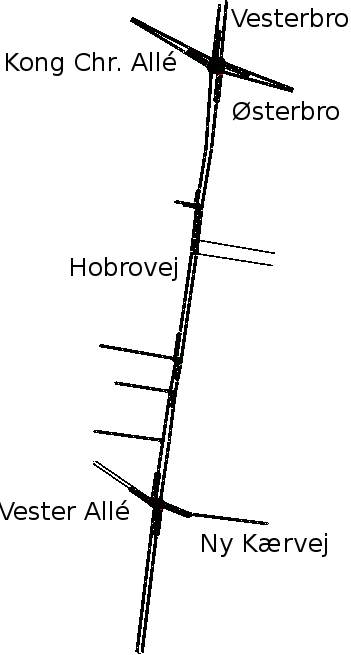
\includegraphics[width=0.15\textwidth]{../images/Hobrovej.png}
\caption{Use case}
\label{fig:Introduction:hobro}
\end{figure}

Hobrovej has seven junctions: two large regulated junctions with $12$ to $16$ connections, two small regulated junctions with $4$ to $6$ connections, and three small unregulated junctions.
The network is an exact replica of Hobrovej, with the same distance between sections and the same number of lanes and connections. 
We have estimated the phases of traffic lights based on local knowledge of the area and a circulation time of 100 seconds.
The routes and the number of vehicles in the network is also based on local knowledge of the area and an OD (Origin-Destination) matrix extracted from GPS trajectories from the project Spar På Farten\cite{}.
We only model vehicles of the types detailed in Tabel~\ref{tabel:vehicleTypes}, and do not model neither pedestrians nor cyclists.

In the following, we will focus our tests on the route going from the south end of Hobrovej to the north end of Hobrovej.
%TODO: Why